To validated that the cluster gives us an improvement when working on big data, a list of tests will be explored. In this section these tests and their results will be presented and evaluated.

\subsection{Best machine learning technique}
\usetikzlibrary{arrows,intersections}
First the best machine learning technique needs to be identified. In this test five different methods were included, these were: naive bayes, hidden naive bayes, logistic regression, neural network and adaboost. All the different methods were tested with multiple parameter settings, however both of the bayes networds has no modifiable parameters.
\begin{figure}[!htb]
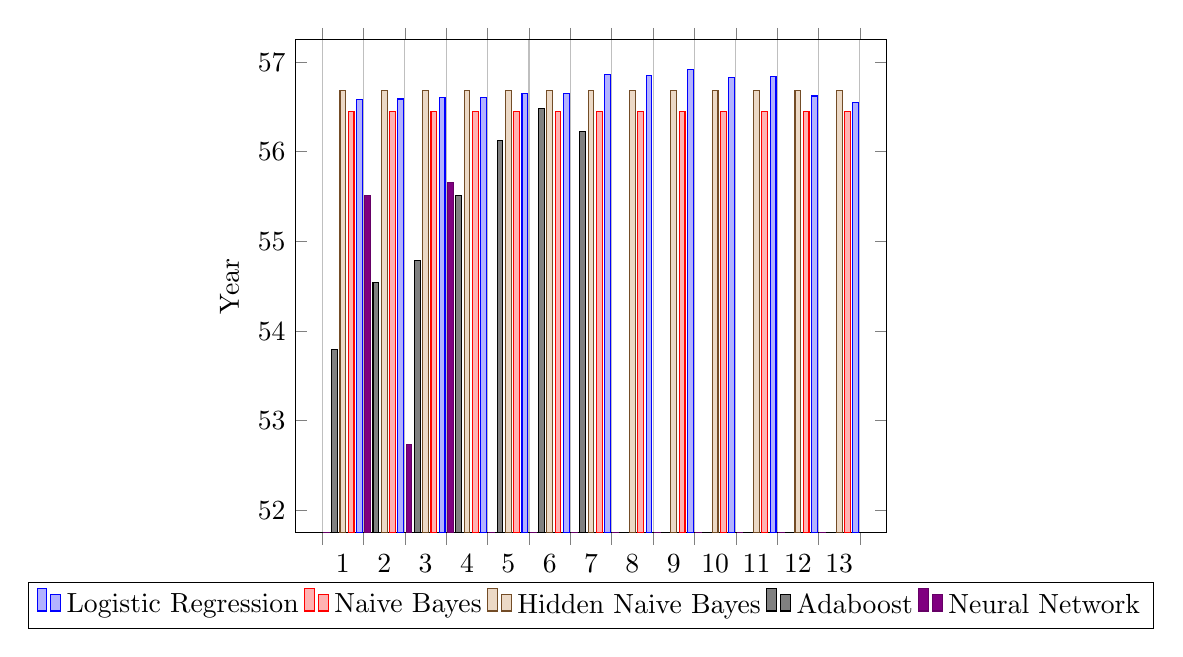
\begin{tikzpicture}
\begin{axis}[
	x tick label style={
		/pgf/number format/1000 sep=},
	ylabel=Year,
	enlargelimits=0.05,
	legend style={at={(0.5,-0.1)},
	anchor=north,legend columns=-1},
	ybar interval=0.7,
        width=.75\textwidth,
        ymin=52, ymax=57,
]
\addplot coordinates {(13,56.5462) 
                      (12,56.6218) 
                      (11,56.8403) 
                      (10,56.8319) 
                      (9,56.916) 
                      (8,56.8487) 
                      (7,56.8655) 
                      (6,56.6471) 
                      (5,56.6471) 
                      (4,56.605) 
                      (3,56.605) 
                      (2,56.5882) 
                      (1,56.5798) 
                      (0,2)};
\addplot coordinates {(13,56.4454) 
                      (12,56.4454) 
                      (11,56.4454) 
                      (10,56.4454) 
                      (9,56.4454) 
                      (8,56.4454) 
                      (7,56.4454) 
                      (6,56.4454) 
                      (5,56.4454) 
                      (4,56.4454) 
                      (3,56.4454) 
                      (2,56.4454) 
                      (1,56.4454) 
                      (0,56.4454)};
\addplot coordinates {(13,56.6807) 
                      (12,56.6807) 
                      (11,56.6807) 
                      (10,56.6807) 
                      (9,56.6807) 
                      (8,56.6807) 
                      (7,56.6807) 
                      (6,56.6807) 
                      (5,56.6807) 
                      (4,56.6807) 
                      (3,56.6807) 
                      (2,56.6807) 
                      (1,56.6807) 
                      (0,56.6807)};
\addplot coordinates {(13,0) 
                      (12,0) 
                      (11,0) 
                      (10,0) 
                      (9,0) 
                      (8,49.87) 
                      (7,56.2269) 
                      (6,56.479) 
                      (5,56.1261) 
                      (4,55.5126) 
                      (3,54.7899) 
                      (2,54.5378) 
                      (1,53.7983) 
                      (0,2)};
\addplot coordinates {(13,0) 
                      (12,0) 
                      (11,0) 
                      (10,0) 
                      (9,0) 
                      (8,0) 
                      (7,0) 
                      (6,0) 
                      (5,50.1) 
                      (4,55.6555) 
                      (3,52.7311) 
                      (2,55.5126) 
                      (1,50.2101) 
                      (0,2)};
\legend{Logistic Regression,Naive Bayes,Hidden Naive Bayes,Adaboost,Neural Network}
\end{axis}
\end{tikzpicture}
\end{figure}

\subsection{Implementation comparison}
To test if Apache Sparks PySpark implementation of logistic regression is implemented properly, it was compared to Weka's and R's implementation equivalent implementation. The dataset consisted of 5000 matches where Weka used the sparse version, R the dense and PySpark on a file with JSON elements. And as seen in \Cref{tab:impl_results}, the implementations are close to equal, the minor differences could be caused by differences in the parameter settings. However these results confirm that Apache Sparks implementation is acceptable. 

\begin{table}[!htb]
  \centering
  \begin{tabular}{|l|c|}
    \hline
    Implementation  & Training error  \\
    \hline
    Weka & 55\%  \\
    R & 55\%\\
    PySpark & 53\%\\ 
    \hline
  \end{tabular}
  \caption{Implementation comparison results}
  \label{tab:impl_results}
\end{table}

\FloatBarrier
\subsection{Feature representation test}
Finding the best way to represent the features. \Cref{sec:representationoffeatures} 

\subsection{Feature tests}
Finding the features that would give the best result.

\subsection{Big data improvements}
Using the same features but an increasing dataset to figure out if big data gives us a better classifier.

\subsection{Speed up}
This test is constructed to test what an increasing number of nodes does to the computation speed. As seen in \Cref{sec:clustersetup}, the cluster consists of 4 nodes, this means the test will be run with the master and either 1, 2 or 3 nodes. The data set will for this test be the same to make the results comparable.










%%% Local Variables:
%%% mode: latex
%%% TeX-master: "../main"
%%% End:
